%%%%% SEC: EMPIRICS
\section{Empirics: Interviews}
\begin{frame}[noframenumbering,c]{Roadmap}
	\tableofcontents[currentsection]
\end{frame}

% SUBSEC:
\subsection{The Northern expedition of 1882}

\begin{frame}{The Northern expedition of 1882}	
	TBD. 	
\end{frame}

% SUBSEC:
\subsection{Glenn Gould's idea of North}

\begin{frame}{Glenn Gould's idea of North}
	TBD.
\end{frame}

% SUBSEC:
\subsection{The U.S. price-to-rent ratio}

\begin{frame}{A figure on a slide}
	\centering
	% Placeholder shipped with the template (assets/placeholders/). Root-anchored path:
	% ../../ climbs from writing/slides/ to the repo root. Swap for your own output/... .
	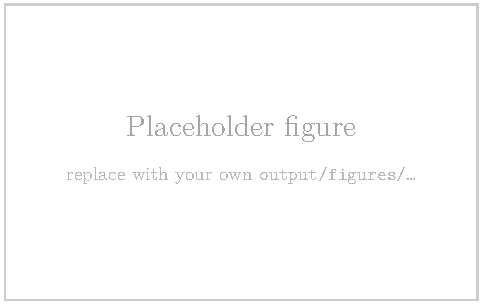
\includegraphics[width=0.5\textwidth]{../../assets/placeholders/placeholder-figure.pdf}

	{\footnotesize Placeholder. Replace the path with an \texttt{output/figures/...}
	artifact and write your own note and \textit{Source:} here.}
\end{frame}

\begin{frame}{A table on a slide}
	\centering
	% Placeholder booktabs fragment shipped with the template (assets/placeholders/).
	% Root-anchored path: ../../ climbs from writing/slides/ to the repo root. The house
	% \input pattern; \small keeps a multi-panel fragment on one slide. Swap for your own.
	\small
	% placeholder-table.tex — a neutral booktabs fragment shipped with the template.
%
% A bare tabular in the house style (\doublerule top, \midrule rules), matching what
% code/analysis exports. The demo \housetable/\input calls in writing/ point here on a
% freshly scrubbed project so the docs compile before any real table exists. Replace with
% your own output/tables/... and repoint the doc.
\begin{tabular}{l*{3}{c}}
\doublerule
                &      (1)&      (2)&      (3)\\
\midrule
Row A           &    0.000&    0.000&    0.000\\
Row B           &    0.000&    0.000&    0.000\\
Row C           &    0.000&    0.000&    0.000\\
\midrule
\end{tabular}


	\vskip\slideblockgap
	{\footnotesize Placeholder. Replace the path with an \texttt{output/tables/...}
	fragment and write your own note here.}
\end{frame}
